\paragraph{}
Durante todo el desarrollo del proyecto, han ido aparenciendo diversas dificultades y problemas que se debieron ir
resolviendo para el correcto y continuo avance del proyecto.

\paragraph{}
Por lo que en este capítulo se exlicarán las distintas soluciones para los principales problemas encontrados. 

%%%%%%%%%%%%%%%%% MOVIMIENTO COCHE %%%%%%%%%%%%%%%%%%%%
%\section{Movimiento vehículo}

\section{Carga desde ficheros}

\paragraph{}
Desde un primer momento se penso en realizar el videojuego de forma que fuera facilmente ampliable siguiendo un manual adecuado, 
donde se explicaran todos los pasos necesarios \footnote{En el apendice de este documento están los distintos manuales para
añadir personajes y circuitos}.

\paragraph{}
Para ello se optó por realizar toda la carga de circuitos, personajes e interfaces de los menús desde archivos. El formato de 
dichos archivos sería XML.

\paragraph{}
De esta forma cualquier persona ya sea programador o no, podrá modificar aspectos tan sencillos como el posicionamiento de los 
botones en lo menús, y las distintas imagenes que pueden aparecer en estos. Respecto a los personaje podrán modificar las 
características de estos, las imagenes que los representan o añadir nuevos personajes. En los circuitos podremos modificar objetos
que aparezcan en estos, así como obstáculos o aparición de ítems.

\paragraph{}
Un ejemplo de fichero XML con la configuración de un menú se puede ver a continuación:

\begin{lstlisting}[style=XML]
<mainmenu background="background_menu" cursor="cursor.xml" 
music='la maryjane - bob wizman.ogg'>
    <title text="Menu Principal" font="cheesebu" size="30" r="0" g="0" b="0" 
    x="15" y="15"/>
    <images>
        <image image_code="separator_line" x="0" y="240"></image>
        <image image_code="logo_menu" x="130" y="5"></image>
    </images>
    <options>
        <option xml_file="menu/mainoption2.xml" font="cheesebu" text="Carrera Rapida" 
        center="True" x="400" y="295"></option>
        <option xml_file="menu/mainoption1.xml" font="cheesebu" text="Campeonato" 
        center="True" x="400" y="335"></option>
        <option xml_file="menu/mainoption2.xml" font="cheesebu" text="Contrarreloj" 
        center="True" x="400" y="400"></option>
        <option xml_file="menu/mainoption1.xml" font="cheesebu" text="Opciones" 
        center="True" x="400" y="440"></option>
        <option xml_file="menu/mainoption2.xml" font="cheesebu" text="Creditos" 
        center="True" x="400" y="505"></option>
        <option xml_file="menu/mainoption1.xml" font="cheesebu" text="Salir" 
        center="True" x="400" y="545"></option>
    </options>
</mainmenu>
\end{lstlisting}

\paragraph{}
Como podemos ver podemos modificar las imagenes que aparecen en el menú o las posiciones de los botones.
En el código únicamente deberiamos dar funcionalidad a cada uno de las opciones del menú.

\paragraph{}
Otro ejemplo de archivo de XMl para los personajes que aparecen en el juego sería el siguiente:

\begin{lstlisting}[style=XML]
<car name_character="Camaro Bun" sprite_code="yellow" max_speed="6.1" 
min_speed="3" aceleration="0.5" desaceleration="0.08" rotation_angle="0.35" 
avatar="avatar1" racer_image='car1'>
<!--NORMAL, NOACTION, RUN, FORWARD, REVERSE, DAMAGED, ERASE, YAW-->
    <animations>
        <animation name="normal" frames="0" delay="1"/>
        <animation name="noaction" frames="0" delay="1"/>
        <animation name="foward" frames="0" delay="1"/>
        <animation name="run" frames="0" delay="1"/>
        <animation name="reverse" frames="0" delay="1"/>
        <animation name="damaged" frames="0" delay="1"/>
        <animation name="erase" frames="0" delay="1"/>
        <animation name="yaw" frames="0" delay="1"/>
        <animation name="fall" frames="0" delay="1"/>
        <animation name="turbo" frames="0" delay="1"/>
    </animations>
</car>
\end{lstlisting}

\paragraph{}
Como podemos ver se pueden modificar los aspectos más básico del comportamiento de los personajes, como pueden ser la velocidad 
máxima de este, velocidad en marcha atrás, aceleración, desaceleración y angulo de giro. También todas las imagenes que representan
al jugador.

\paragraph{}
Incluso si la imagen del coche del personaje es un sprite podemos indicar que frames de este pertencen a cada uno de los posibles 
estados del personaje.

%%%%%%%%%%%%%%%%% CIRCUITOS %%%%%%%%%%%%%%%%%%%%%%%%%
\section{Formato y carga de circuitos}

\paragraph{}
Una de las primeras dudas que surgieron al poco tiempo de comenzar el desarrollo de \emph{Zycars}, fue el formato que deberían
tener los distintos circuitos o niveles que aparecerían a lo largo del juego. Para ellos tenía varias alternativas:

\begin{itemize}
    \item \textbf{Opción 1}: los circuitos estarían compuestos por una única imagen realizada previamente. En un fichero aparte se 
    podría indicar las zonas colisionables que tendría la imagen u otras características relevantes.
    
    \item \textbf{Opción 2}: crear los circuitos mediante un sistema de tiles, de formas que en un fichero de texto plano, indicaramos 
    los tieles que componen el circuito, así como la característica de estos.
    
    \item \textbf{Opción 3}: usar algún software que nos permitiera la creación y edición de niveles, de forma sencilla, mediante tiles.
\end{itemize}

\paragraph{}
Finalmente se optó por la opción 3, para ello se usó el programa \emph{Tiled} \footnote{Se comenta su uso y características en el
apéndice relacionado con las herramientas utilizadas}, dicho programa me proporcionaba todas las necesidades básicas, como una 
sencilla edición y creación de niveles, así como la gestión de capas, para poder poner elementos en el circuito a un nivel 
superior o inferior. Para ello se debia crear una imagen con todos los tiles que compondrían un circuito.

\paragraph{}
Este programa generaba como resultado un archivo \emph{XML}, que se procesaría posteriormente en tiempo de ejecución. También hay
que añadir que esta opción elegida era una de las que menos nos ocuparía en memoria, ya que no es lo mismo tener un circuito 
completo en una única imagen, dicha imagen sería demasiado grande y ocuparía bastante memoria. Mientras
que con esta opción tendriamos una imagen pequeña con el conjunto necesario de tiles para el circuito en cuestión.

\paragraph{}
El formato de los XML generados por el programa son de la siguiente forma:

\begin{lstlisting}[style=XML]
<?xml version="1.0" encoding="UTF-8"?>
<map version="1.0" orientation="orthogonal" width="88" height="74" tilewidth="45" tileheight="45">
 <properties>
  <property name="ancho_meta" value="5"/>
  <property name="ancho_pista" value="5"/>
  <property name="collision_map" value="collisionmapgarden.png"/>
  <property name="grado_coche" value="270"/>
  <property name="tileset_alto" value="35"/>
  <property name="tileset_ancho" value="21"/>
 </properties>
 <tileset firstgid="1" name="tilesetgarden" tilewidth="45" tileheight="45">
  <image source="tilesetgarden.png" width="945" height="1575"/>
 </tileset>
 <layer name="Capa 1" width="88" height="74">
  <data>   
   <tile gid="1"/>
   <tile gid="2"/>
   ....
  </data>   
 </layer>
 <layer name="Capa 2" width="88" height="74">
  <data>
   <tile gid="0"/>
   <tile gid="0"/>
   ...
 </layer>
 <layer name="Capa 3" width="88" height="74">
  <data>
   <tile gid="74"/>
   <tile gid="75"/>
   ...
  </data>
 </layer>
 <objectgroup name="checkpoints" width="88" height="74" opacity="0.2">
  <object name="1" type="Horizontal" x="180" y="1035" width="45" height="45"/>
  <object name="1" type="check" x="450" y="225" width="45" height="45"/>
  <object name="2" type="check" x="2205" y="405" width="45" height="45"/>
 </objectgroup>
</map>
\end{lstlisting}

\paragraph{}
Una de las únicas cosas que no propocionaba el programa era poder indicar cuales de los tiles eran colisionables, atravesables o
de cualquier otro tipo. Así que para solventar este problema se elijió tener a parte de la imagen que contendría el conjunto de 
tiles otra imagen con las mismas características, como tamaño y el tamaño de los tiles, solo que esta ultima lo tiles tendrían 
colores planos indicando de que tipo serían. Así cuando cargaramos el circuito que necesitaramos en ese momento y con ello
el conjunto de tiles relacionado, se comprobaría que color tiene cada uno de los tiles en la otra imagen y así almacenar
de que tipo son. A continuación se muestran dos imagenes como ejemplo:

\begin{itemize}

    \item Este sería el aspecto de una imagen con el conjunto de tiles necesarios:
    \begin{figure}[H]
      \label{tileset}
      \begin{center}
        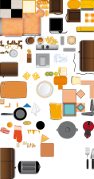
\includegraphics[scale=1.45]{imagenes/tileset.png}
      \end{center}
      \caption{Implementación: conjunto de tiles}
    \end{figure}
    
    \item Y esta la imagen que indicaría de que tipo son cada uno de los tiles de la imagen anterior:
    \begin{figure}[H]
      \label{collisionmap}
      \begin{center}
        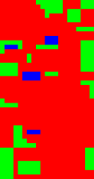
\includegraphics[scale=1.45]{imagenes/collisionmap.png}
      \end{center}
      \caption{Implementación: Mapa de colisiones}
    \end{figure}
    
\end{itemize}

\paragraph{}
Como se puede apreciar la segunda imagen tiene las mismas características que la superior, solo que los tiles que contiene
son de un único color para indicar el tipo de los tiles. Los tipos de tiles que se eligieron añadir fueron los siguientes:

\begin{itemize}
    \item \textbf{Rojo}: tiles completamentes atravesables, su única función es decorativa.
    
    \item \textbf{Verde}: tiles colisionables, aquellos que no pueden ser atravesados, normalmente marcan el recorrido
    del circuito, también usados como obstáculos.
    
    \item \textbf{Azul}: tiles atravesables, pero realentizan de forma considerable al vehículo que pase sobre ellos.
\end{itemize}

\section{Colisiones}

\paragraph{}
La detección de las colisiones es una de las cosas más básicas de la mayoría de los juegos en la que los jugadores
recorren mapas o niveles.

\paragraph{}
En \emph{Zycars} debemos de gestionar varios tipos de colisiones, entre esos tipos estaría la colisión que se produciría 
entre cualquier vehículo y el escenario en el que se encuentre, así como la colisión entres dos objetos del juego, como podrían
ser desde dos vehículos entre si, o algún vehículo por algun item lanzado por otro jugador.

\paragraph{}
Indicar que cada uno de los objetos que intervienen en el juego y puede colisionar con cualquier elemento, tienen
un rectangulo asociado a su forma, de manera que sea más sencilla la detección de colisiones.

\paragraph{}
En las siguiente subsecciones se explicará cuales son las soluciones que se llevaron a cabo para la gestión de las colisiones 
en cada una de las situaciones posibles.

\subsection{Colisión con el escenario}

\paragraph{}
Como se comento en el apartado dedicado a la carga y formato de los circuitos, cada uno de los circuitos tiene asociado una imagen
que indica de que tipo es cada uno de los tiles que nos podemos encontrar a lo largo del circuito.

\paragraph{}
Así que a la hora de cargar el circuito en el que vayamos a competir almacenabamos cada uno de los tiles que componían el circuito,
así como el tipo que eran. Dada esta situación debemos ir comprobando si el jugador esta atravensando algún tile colisionable. 
Si es el caso debemos corregir la posición del objeto con respecto al tile con el que estaba colisionando.

\paragraph{}
A la hora de realizar la correción de la colisión, debemos tener en cuenta aspectos como, ángulo del vehículo, dirección del 
vehículo, así como el lado del tile por el que se produce la colisión, ya sea por la parte superior, inferior o alguno 
de los laterales. Según estos parámetros la collisión se corregirá en una dirección u otra.

\paragraph{}
A continuación se expone un ejemplo visual para su correcta comprensión:

\begin{itemize}
    \item Se detecta que un vehículo colisiona con un tile colisionable:
    \begin{figure}[H]
      \label{colision1}
      \begin{center}
        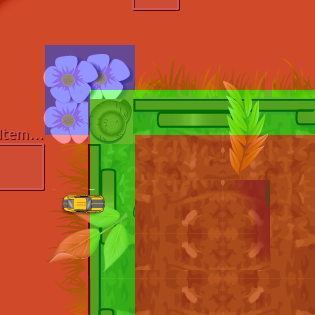
\includegraphics[scale=0.7]{imagenes/colision1.png}
      \end{center}
      \caption{Implementación: Colisión con el escenario 1/2}
    \end{figure}
    
    \item Se corrige la colisión en función del ángulo y dirección del vehículo, asi como el lado por el que colisiona del tile:
    \begin{figure}[H]
      \label{colision2}
      \begin{center}
        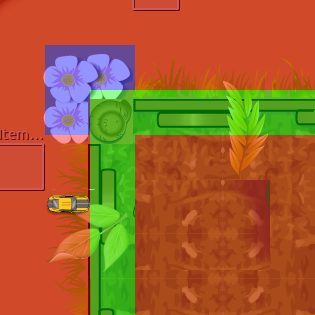
\includegraphics[scale=0.7]{imagenes/colision2.png}
      \end{center}
      \caption{Implementación: Colisión con el escenario 2/2}
    \end{figure}
    
\end{itemize}

\paragraph{}
En el caso de que se colisione con un tile que atravesable pero era del tipo que realentizaban la velocidad, únicamente
se reducirá la velocidad del vehículo y no se corregira su posición para este tile.


\subsection{Colisiones entre objetos}

\paragraph{}
En este caso hay varias posibilidades según que tipos de objetos han colisionado, en todas ellas la detección de la colisión
se hace de forma similar, comprobamos si alguna de las caja de colisiones de los objetos en cuestión se superponen o no.

\paragraph{}
A continuación se exponen las distintas situaciones que pueden suceder:

\begin{itemize}
    \item \textbf{Colisión vehículo-vehículo}: dos vehículos en carrera colisionan entre sí, en este caso debemos comprobar 
    cual de los dos vehículos ha colisionado con el otro, es decir, cual se ha interpuesto. En ese caso 
    corregiremos la posición de ese vehículo y produciremos algún tipo de rebote en función de la velocidad que llevara
    en ese momento.
    
    \item \textbf{Colisión vehículo-item}: en este caso se responderá a la colision dependiendo del tipo de item con el que
    hemos colisionado.
    \begin{itemize}
        \item Si el item es un misil o una bola, el item pasará a su estado de explosión, mientras que el vehículo parasa a un estado de daño
        
        \item Si el item es una mancha de aceite, el item no cambiará su estado, pero el coche pasar a un estado de descontrol durante
        unos instantes
        
        \item Si el item es un chicle, se reducirá de forma considerable la velocidad del vehículo.
    \end{itemize}
\end{itemize}

%%%%%%%%%%%%%%%%%%%% INTELIGENCIA ARTIFICIAL %%%%%%%%%%%%%%%%%%%%%%%%
\section{Inteligencia artificial}

\paragraph{}
Otro de los aspectos más importante de un videojuego de las carácteristicas de \emph{Zycars}, es la inteligencia artificial,
ya que en dos de los tres modos de juegos disponibles el objetivo es obtener la mejor clasificación posible, por delante
de los demás coches manejados por la inteligencia artificial.

\paragraph{}
Entre las habilidades que debe tener la inteligencia artificial deben ser:

\begin{itemize}
    \item \textbf{Realización del recorrido}: la inteligencia artificial debe ser capaz de realizar los recorridos de los
    circuitos.
    
    \item \textbf{Lanzamiento de items}: también debe poder tirar los items que reciba de las bolas de items.
\end{itemize}

\paragraph{}
En los siguientes apartados se explicará de que forma se han afrontado los distintos problemas para obtener una inteligencia
artificial que cumpla las espectativas básicas.

\subsection{Realización del recorrido. Algoritmo de búsqueda A*}

\paragraph{}
Esta es la parte más importante de la inteligencia artificial, ya que en un juego de conducción y carreras, lo mínimo que se 
espera es que la inteligencia artificial realice los recorridos de los circuitos disponibles, con el objetivo de vencer al
jugador.

\paragraph{}
A lo largo de los circuitos existen unos puntos de control que cada uno de los vehículo de la inteligencia artificial
debe pasar para realizar la vuelta al circuito, dichos puntos de control ocupan un tile.

\paragraph{}
Para ello, aprovechando que tenemos un circuito creado por tiles y que podemos saber en todo momendo en el tile actual
que se puede encontrar cualquiera de los competidores, se decidió que se implementaría el algoritmo de búsqueda A*.

\subsubsection{Algoritmo de búsqueda A*}

\paragraph{}
El objetivo del algoritmo A* es buscar el camino más corto y óptimo, en el caso de que exista, desde un nodo origen, hasta un
nodo destino. A la hora de buscar dicho camino se tienen en cuenta factores como, el valor heurístico que poseen cada uno
de los nodos, así como el coste real del recorrido.

\paragraph{}
Dicho algoritmo tiene la siguiente función de evaluación f(n) = g(n) + h'(n), siendo h'(n) el valor heurístico del nodo actual n,
hasta el final y g(n) el coste real del camino desde el origen al nodo actual.

\begin{figure}[H]
  \label{a_star}
  \begin{center}
    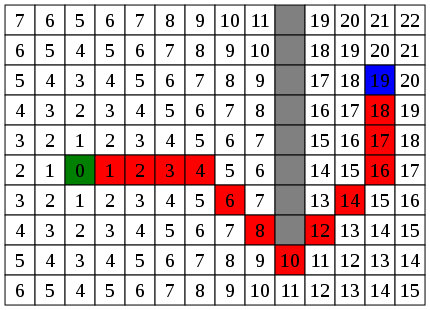
\includegraphics[scale=0.6]{imagenes/a_star.png}
  \end{center}
  \caption{Implementación: Ejemplo del algoritmo A*}
\end{figure}

\paragraph{}
En el A* se tiene dos estructuras diferencidas:

\begin{itemize}
    \item Lista de abiertos: donde se encuentran los nodos por los que aún no se han pasado
    \item Lista de cerrados: donde se encuentran los nodos por los que ya se han pasado
\end{itemize}

\paragraph{}
El funcionamiento general del algoritmo es el siguiente, partiendo de un nodo en el que nos encontramos actualmente,
obtenemos todos los nodos vecinos de este, comprobamos que no se encuentren en la lista de abiertos, ni en la lista
de cerrado para evitar ciclos, todos aquellos que cumplan dichos requisitos se añaden a la lista de abiertos. En el caso de que 
alguno de los nodos se encuentren en la lista de abiertos, comparamos el valor de f(n), en el caso de que sea menor lo 
sustituiremos. Una vez evaluado dicho nodo, pasamos a obtener de la lista de abiertos aquel nodo que tenga un f(n) menor y 
comenzamos de nuevo todo el proceso anterior. En el momento en el que llegemos al nodo objetivo, detenemos la búsqueda y devolvemos
el camino completo.

\paragraph{}
Dicho algoritmo se aplica en \emph{Zycars}, de forma que el vehículo controlado por la inteligencia artificial, tiene todos los
puntos de chequeo, en orden, que debe atravesar para recorrer el circuito completo. Así que en cada momento se comprobará
el tile actual en el que se encuentra y se obtendrá el camino más óptimo y corto hasta el siguiente punto de chequeo, una vez
llegado a este se hará una nueva consulta al A* para obtener el camino al próximo y así sucesivamente.

\subsection{Lanzamiento de items.}

\paragraph{}
La inteligencia artificial debe ser capaz de lanzar los items disponibles a los largo del juego, según las distintas 
situaciones en la que se encuentre, en el momento que obtenga dicho item.

\paragraph{}
Por ejemplo, cuando obtenga un misil o una bola deberá lanzarlos en el momento que tenga algún oponente delante y a tiro. Pero si
en cambio hemos obtenido como item una macha de aceite o un chicle, deberá lanzarlo en el momento que tenga un oponente detrás
y lo más cerca posible para que no tenga tiempo para maniobrar y poder esquivar el obstaculo.

\paragraph{}
Como solución, se eligió una forma muy sencilla y eficiente a la hora de realizarlo. Para ello cada vehículo controlado por la
inteligencia artificial, tiene tanto un segmento que va desde el centro del coche hacia unos pixeles por delante de la posición
actual del vehículo, como otro segmento que también va desde el centro pero uno pixeles atrás de la posición del vehículo. 
Si se pudieran ver dichos segmente, tendrían la siguiente forma:

\begin{figure}[H]
  \label{ia_segmentos}
  \begin{center}
    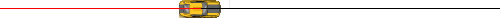
\includegraphics[scale=0.8]{imagenes/ia_segmentos.png}
  \end{center}
  \caption{Implementación: Segmentos de la inteligencia artificial}
\end{figure}

\paragraph{}
De forma que en el momento que tengamos un item que se lanza por la parte delantera del vehículo, se comprobará si alguno de los 
oponentes colisiona con la barra delantera de este. En el caso de que tengamos un item que se lanza por la parte trasera, haríamos
la misma comparación pero con la barra trasera.
